\testCom
{%Номер задачи
	3.213
}
{%Условие
	условие
}
{%Дано
	дано
}
{%Найти
	найти
}
{%Решение
	%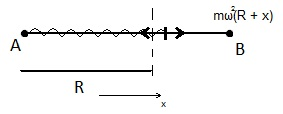
\includegraphics[height=30mm]{3_33.jpg}\\
	%$dE = dE_к + dE_п = \frac{p S}{2} (\dot \xi^2 + \upsilon^2 (\pder{\xi}{x}{})^2)\, dx$\\
	$E = \frac{pS}{2} \int\limits_0^{\frac{\lambda}{2}} (a^2 \omega^2 \sin^2 \omega t + a^2 k^2 \upsilon^2 \cos^2 k x \cos^2 \omega t) dx = \left[ \frac{\lambda}{2} = \frac{\upsilon}{2 \nu} = \frac{\upsilon \cdot 2 \pi}{2 \omega} = \frac{\pi}{k}\right] = $\\
	$= \frac{pS}{2} \left(\frac{a^2 \omega^2 \pi}{2k} \sin^2 \omega t + \frac{a^2 k^2 \pi \upsilon^2}{2 k} \cos^2 \omega t \right) = \frac{pS a^2 \pi}{4 k} \left(\omega^2 \sin^2 \omega t + (k \upsilon)^2 \cos^2 \omega t \right) = \frac{\rho S a^2 \omega^2 \pi}{4 k}$\\
}

